\section{Example: A regional model of the Jakobshavn outlet glacier in Greenland}\label{sec:jako} \index{Jakobshavn} \index{PISM!regional model example}
\optsection{Jakobshavn}

Jakobshavn Isbrae is a fast-flowing outlet glacier in western Greenland that drains approximately 7\% of the area of the Greenland ice sheet.  It experienced a large acceleration following the loss of its floating tongue in the 1990s \cite{JoughinAbdalatiFahnestock}, an event which seems to have been driven by warmer ocean temperatures \cite{Hollandetal2008}.  Because it is thick, has a steep surface slope, has a deep trough in its bedrock topography (Figure \ref{fig:jako-basin-topg}), and has a thick layer of low-viscosity temperate ice at its base \cite{Luethietal2009}, this ice flow is different from the ice streams in West Antarctica or Northeast Greenland \cite{TrufferEchelmeyer}.
 
This section describes how to build a PISM regional model of this outlet glacier \cite{DellaGiustina2011} using scripts from \texttt{examples/jako/}.  The same strategy should work for other outlet glaciers.  We also demonstrate the PISM executable \texttt{pismo} (``outlet-glacier mode''), and Python drainage-basin-delineation tools \href{https://github.com/pism/regional-tools}{\texttt{regional-tools}} which can be downloaded from the PISM source code website.  Such regional models allow modest-size computers to run high resolution models\footnote{PISM can also do 1\,km runs for the whole Greenland ice sheet; see this \href{http://www.pism-docs.org/wiki/doku.php?id=news:first1km}{news item}.} and large ensembles.  Regional analysis is justified if detailed data is available for the region.\index{PISM!pismo executable for outlet glaciers}\index{regional-tools}

\index{CReSIS bedrock topography for Jakobshavn}
The geometric data used here is the SeaRISE  \cite{Bindschadler2013SeaRISE} 1\,km dataset for the whole Greenland ice sheet.  It contains bedrock topography from recent CReSIS radar in the Jakobshavn area.  We also use the SeaRISE 5\,km data set which has climatic mass balance from the Greenland-region climate model RACMO \cite{Ettemaetal2009}.

A regional ice flow model generally needs ice flow and stress boundary conditions.  For this we use a 5\,km grid, whole ice sheet, spun-up model state from PISM, described in Section \ref{sec:start} of this \emph{Manual}.  You can download the large NetCDF result from the PISM website, or you can generate it by running a Section \ref{sec:start} script. 

\begin{figure}[ht]
  \centering
  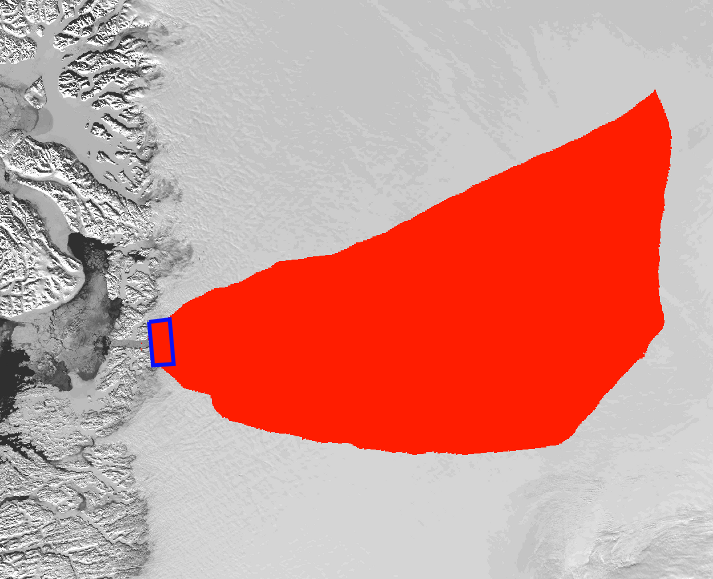
\includegraphics[height=2.1in,keepaspectratio=true]{jako-ftt-mask} \, 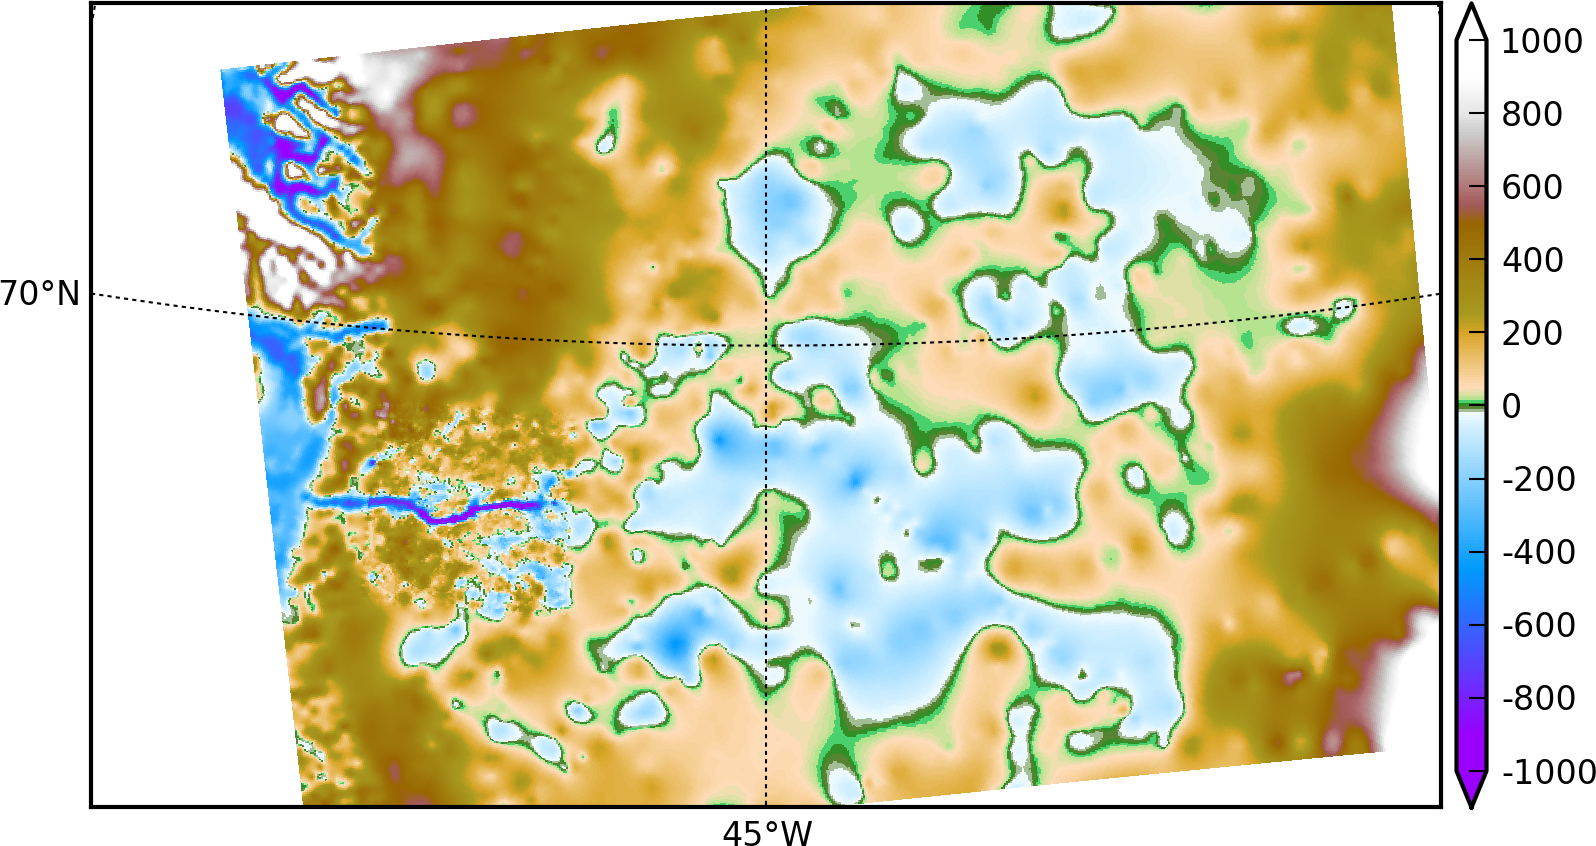
\includegraphics[height=2.1in,keepaspectratio=true]{jako-topg}
  \caption{A \texttt{regional-tools} script computes a drainage basin mask from the surface DEM (left; Modis background) and from a user-identified terminus rectangle (blue).  The regional model can exploit high-resolution bedrock elevations inland from Jakobshavn fjord (right; meters asl).}
  \label{fig:jako-basin-topg}
\end{figure}


\subsection*{Get the drainage basin delineation tool}
The drainage basin tool \texttt{regional-tools} is at \url{https://github.com/pism/regional-tools}.  Get it using \texttt{git} and set it up as directed in its \texttt{README.md}.  Then come back to the \texttt{examples/jako/} directory and link the script.  Here is the quick summary:
\begin{quote}\small
\begin{verbatim}
$ cd ~/usr/local/                                      # the location you want
$ git clone https://github.com/pism/regional-tools.git
$ cd regional-tools/
$ python setup.py install                              # may add "sudo" or "--user"
$ cd PISM/examples/jako/
$ ln -s ~/usr/local/regional-tools/pism_regional.py .  # symbolic link to tool
\end{verbatim}
\normalsize\end{quote}

\subsection*{Preprocess the data and get the whole ice sheet model file}
Script \texttt{preprocess.sh} downloads and cleans the 1\,km SeaRISE data, an 80 Mb file called \texttt{Greenland1km.nc}.\footnote{If this file is already present then no actual download occurs, and preprocessing proceeds.  Thus:  Do not worry about download time if you need to preprocess again.  The same comment applies to other downloaded files.}  The script also downloads the SeaRISE 5\,km data set \texttt{Greenland_5km_v1.1.nc}, which contains the RACMO surface mass balance field (not present in the 1\,km data set).  If you have already run the example in Section \ref{sec:start} then you already have this file and you can link to it to avoid downloading:
\begin{quote}\small
\begin{verbatim}
$ ln -s ../std-greenland/Greenland_5km_v1.1.nc
\end{verbatim}
\normalsize\end{quote}

The same script also preprocesses a pre-computed 5\,km grid PISM model result \texttt{g5km_gridseq.nc} for the whole ice sheet.  This provides the boundary conditions, and the thermodynamical initial condition, for the regional flow model we are building.  If you have already generated it by running the script in subsection \ref{subsect:gridseq} then link to it,
\begin{quote}\small
\begin{verbatim}
$ ln -s ../std-greenland/g5km_gridseq.nc
\end{verbatim}
\normalsize\end{quote}
Otherwise running \texttt{preprocess.sh} will download it.  Because it is about 0.6 Gb this may take some time.

So now let's actual run the preprocessing script:
\begin{quote}\small
\begin{verbatim}
$ ./preprocess.sh
\end{verbatim}
\normalsize\end{quote}
Files \texttt{gr1km.nc}, \texttt{g5km_climate.nc}, and \texttt{g5km_bc.nc} will appear.  These can be examined in the usual ways, for example:
\begin{quote}\small
\begin{verbatim}
$ ncdump -h gr1km.nc | less            # read metadata
$ ncview gr1km.nc                      # view fields
\end{verbatim}
\normalsize\end{quote}
The boundary condition file \texttt{g5km_bc.nc} contains thermodynamical spun-up variables (\texttt{enthalpy,bmelt,bwat}) and boundary values for the sliding velocity (\texttt{u_ssa_bc,v_ssa_bc}); these have been extracted from \texttt{g5km_gridseq.nc}.

None of the above actions is specific to Jakobshavn, though all are specific to Greenland.  If your goal is to build a regional model of another outlet glacier in Greenland, then you may be able to use \texttt{preprocess.sh} as is.  The SeaRISE 1\,km data set has recent CReSIS bed topography data only for the vicinity of the Jakobshavn outlet, however, and it is otherwise just BEDMAP.  Because outlet glacier flows are bed-topography-dominated, additional bed elevation data should be sought.

\subsection*{Identify the drainage basin for the modeled outlet glacier}
Here we are going to extract a ``drainage basin mask'' from the surface elevation data (DEM) in \texttt{gr1km.nc}.  The goal is to determine, in part, the locations outside of the drainage basin where boundary conditions taken from the precomputed whole ice sheet run can be applied to modeling the outlet glacier flow itself.

The basin mask is determined by the gradient flow of the surface elevation.  Thus generating the mask uses a highly-simplified ice dynamics model (namely: ice flows down the surface gradient).  Once we have the mask, we will apply the full PISM model in the basin interior marked by the mask.  Outside the basin mask we will apply simplified models or use the whole ice sheet results as boundary conditions.

The script \texttt{pism_regional.py} computes the drainage basin mask based on a user choice of a ``terminus rectangle''; see Figure \ref{fig:jako-basin-topg}.  There are two ways to use this script:
\begin{itemize}
\item \textbf{To use the graphical user interface (GUI) mode.}  Run
\begin{quote}\small
\begin{verbatim}
$ python pism_regional.py
\end{verbatim}
\normalsize\end{quote}
Select \texttt{gr1km.nc} to open.  Once the topographic map appears in the Figure window, you may zoom enough to see the general outlet glacier area.  Then select the button ``Select terminus rectangle''.  Use the mouse to select a small rectangle around the Jakobshavn terminus (calving front), or around the terminus of another glacier if you want to model that.  Once you have a highlighted rectangle, select a ``border width'' of at least 50 cells.\footnote{This recommendation is somewhat Jakobshavn-specific. We want our model to have an ice-free down flow (western) boundary on the resulting computational domain for the modeled region.}  Then click ``Compute the drainage basin mask.''  Because this is a large data set there will be some delay. (Multi-core users will see that an automatic parallel computation is done.)  Finally click ``Save the drainage basin mask'' and save with your preferred name; we will assume it is called \texttt{jakomask.nc}.  Then quit.
\item \textbf{To use the command-line interface.}  The command-line interface of \texttt{pism_regional.py} allows one to re-create the mask without changing the terminus rectangle choice.  (It also avoids the slowness of the GUI mode for large data sets.)  In fact, for repeatability, we will assume you have used this command to calculate the drainage basin:
\begin{quote}\small
\begin{verbatim}
$ python pism_regional.py -i gr1km.nc -o jakomask.nc -x 360,382 -y 1135,1176 -b 50
\end{verbatim}
\normalsize\end{quote}
This call generates the red region in Figure \ref{fig:jako-basin-topg}.  Options \texttt{-x A,B -y C,D} identify the grid index ranges of the terminus rectangle, and option \texttt{-b} sets the border width.  To see more script options, run with \texttt{--help}.
\end{itemize}

\subsection*{Cut out the computational domain for the regional model}
We still need to ``cut out'' from the whole ice sheet geometry data \texttt{gr1km.nc} the computational domain for the regional model.  The climate data file \texttt{g5km_climate.nc} and the boundary condition file \texttt{g5km_bc.nc} do not need this action because PISM's coupling and SSA boundary condition codes already handle interpolation and/or subsampling for such data.

You may have noticed that the text output from running \texttt{pism_regional.py} included a cutout command which uses \texttt{ncks} from the NCO tools.  This command also appears as a global attribute of \texttt{jakomask.nc}:
\begin{quote}\small
\begin{verbatim}
$ ncdump -h jakomask.nc | grep cutout
\end{verbatim}
\normalsize\end{quote}
Copy and run the command that appears, something like
\begin{quote}\small
\begin{verbatim}
$ ncks -d x,299,918 -d y,970,1394 gr1km.nc jako.nc
\end{verbatim}
\normalsize\end{quote}
This command is also applied to the mask file; note the option \texttt{-A} for ``append'':
\begin{quote}\small
\begin{verbatim}
$ ncks -A -d x,299,918 -d y,970,1394 jakomask.nc jako.nc
\end{verbatim}
\normalsize\end{quote}
Now look at \texttt{jako.nc}, for example with ``\texttt{ncview -minmax all jako.nc}''.  This file is the full geometry data ready for a regional model.  The field \texttt{ftt_mask} identifies the drainage basin, outside of which we will use simplified time-independent boundary conditions.  Specifically, outside of the \texttt{ftt_mask} area, but within the computational domain defined by the extent of \texttt{jako.nc}, we will essentially keep the initial thickness.  Inside the \texttt{ftt_mask} area all fields will evolve normally.

\subsection*{Quick start}
The previous steps starting with the command ``\texttt{./preprocess.sh}'' above, then using the command-line version of \texttt{pism_regional.py}, and then doing the \texttt{ncks} cut-out steps, are all accomplished in one script,
\begin{quote}\small
\begin{verbatim}
$ ./quickjakosetup.sh
\end{verbatim}
\normalsize\end{quote}
Running this takes about a minute on a fast laptop, assuming data files are already downloaded.

\subsection*{Spinning-up the regional model on a 5\,km grid}
To run the PISM regional model we will need to know the number of grid points in the 1\,km grid in \texttt{jako.nc}.  Do this:
\begin{quote}\small
\begin{verbatim}
$ ncdump -h jako.nc |head
    netcdf jako {
    dimensions:
      y = 425 ;
      x = 620 ;
    ...
\end{verbatim}
\normalsize\end{quote}
The grid has spacing of 1\,km, so our computational domain is a 620\,km by 425\,km rectangle.  A 2\,km resolution, century-scale model run is easily achievable on a desktop or laptop computer, and that is our goal below.  A lower 5\,km resolution spin-up run, matching the resolution of the 5\,km whole ice sheet state computed earlier, is also achievable on a small computer; we do that first.

The boundary condition fields in \texttt{g5km_bc.nc}, from the whole ice sheet model result  \texttt{g5km_gridseq.nc}, may or may not, depending on modeller intent, be spun-up adequately for the purposes of the regional model.  For instance, the intention may be to study equilibrium states with model settings special to the region.  Here, however we assume that some regional spin-up is needed, if for no other reason that the geometry used here (from the SeaRISE 1km data set) differs from that in the whole ice sheet model state.

We will get first an equilibrium 5\,km regional model, and then do a century run of a 2\,km model based on that.  While determining ``equilibrium'' requires a decision, of course, a standard satisfied here is that the ice volume in the region changes by less than 0.1 percent in the final 100 model years.  See \texttt{ivol} in \texttt{ts_spunjako_0.nc} below.

The 5\,km grid\footnote{Calculate \texttt{620/5 + 1} and \texttt{425/5 + 1}, for example.} uses \texttt{-Mx 125 -My 86}.  So now we do a basic run using 4 MPI processes:
\begin{quote}\small
\begin{verbatim}
$ ./spinup.sh 4 125 86 &> out.spin5km &
\end{verbatim}
\normalsize\end{quote}
You can read the \texttt{stdout} log file while it runs: ``\texttt{less out.spin5km}''.  The run takes about 5 processor-hours on a 2013 laptop.   % 4.5055 proc-hours on bueler-gazelle
It produces three files which can be viewed (e.g.~with \texttt{ncview}): \texttt{spunjako_0.nc}, \texttt{ts_spunjako_0.nc}, and \texttt{ex_spunjako_0.nc}.  Some more comments on this run are appropriate:
\begin{itemize}
\item Generally the regridding techniques used at the start of this spin-up run are recommended for regional modeling.  Read the actual run command by
\begin{quote}\small
\begin{verbatim}
$ PISM_DO=echo ./spinup.sh 4 125 86 | less
\end{verbatim}
\normalsize\end{quote}
\item  We use \texttt{-i jako.nc -bootstrap}, so we get to choose our grid, and (as usual in PISM with \texttt{-bootstrap}) the fields are interpolated to our grid.
\item A modestly-fine vertical grid with 20 m spacing is chosen, but even finer is recommended, especially to resolve the temperate ice layer in these outlet glaciers.
\item There is an option \intextoption{no_model_strip} \texttt{10} asking \texttt{pismo} to put a 10\,km strip around edge of the computational domain.  This strip is entirely outside of the drainage basin defined by \texttt{ftt_mask}.  In this strip the thermodynamical spun-up variables \texttt{bmelt,tillwat,enthalpy,litho_temp} from \texttt{g5km_bc.nc} are held fixed and used as boundary conditions for the conservation of energy model.  A key part of putting these boundary conditions into the model strip are the options
\begin{quote}\small
\begin{verbatim}
  -regrid_file g5km_bc.nc -regrid_vars bmelt,tillwat,enthalpy,litho_temp,vel_ssa_bc
\end{verbatim}
\normalsize\end{quote}
\item Dirichlet boundary conditions \texttt{u_ssa_bc,v_ssa_bc} are also regridded from \texttt{g5km_bc.nc} for the sliding SSA stress balance, and the option \texttt{-ssa_dirichlet_bc} then uses them during the run.  The SSA equations are solved as usual except in the \texttt{no_model_strip} where these Dirichlet boundary conditions are used.  Note that the velocity tangent to the north and south edges of the computational domain is significantly nonzero, which motivates this usage.
\item The calving front of the glacier is handled by the following option combination:
\begin{quote}\small
\begin{verbatim}
   -calving ocean_kill -ocean_kill_file jako.nc -pik
\end{verbatim}
\normalsize\end{quote}
This choice uses the present-day ice extent, defined by SeaRISE data in \texttt{Greenland1km.nc}, to determine the location of the calving front.  Recalling that \texttt{-pik} includes \texttt{-cfbc}, we are applying a PIK mechanism for the stress boundary condition at the calving front.  The other PIK mechanisms are largely inactive because of \texttt{-calving ocean_kill}, but they should do no harm (see section \ref{sec:pism-pik}).
\end{itemize}

\begin{figure}[ht]
  \centering
  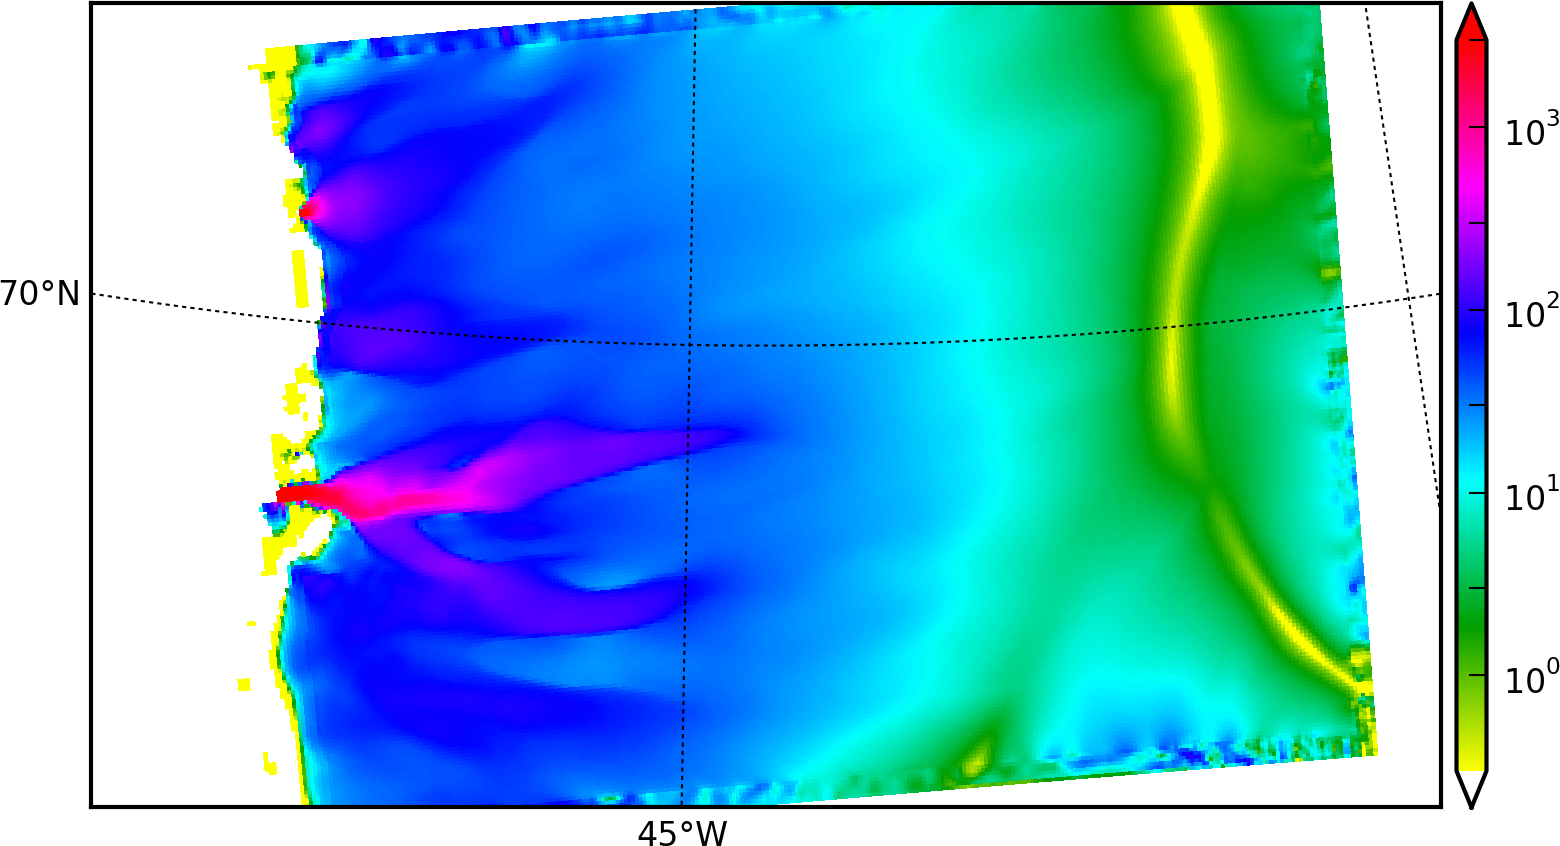
\includegraphics[width=1.05\textwidth,keepaspectratio=true]{jako-csurf}
  \caption{Left: modeled surface speed at the end of a 2\,km grid, 100 model year, steady present-day climate run.  Right: observed surface speed, an average of four winter velocity maps (2000,2006--2008) derived from RADARSAT data, as included in the SeaRISE  5\,km data set \cite{Joughinetal2010}, for the same region.  Scales are in meters per year.}
  \label{fig:jako-csurf}
\end{figure}


\subsection*{Century run on a 2\,km grid}
Now that we have a spun-up state, here is a 100 model year run on a 2\,km grid with a 10 m grid in the vertical:
\begin{quote}\small
\begin{verbatim}
$ ./century.sh 4 311 213 spunjako_0.nc &> out.2km_100a &
\end{verbatim}
\normalsize\end{quote}
This run requires at least 6\,GB of memory, and it takes about 16 processor-hours.

It produces a file \texttt{jakofine_short.nc} almost immediately and then restarts from it because we need to regrid fields from the end of the previous 5\,km regional run (in \texttt{spunjako_0.nc}) and then to ``go back'' and regrid the SSA boundary conditions from the 5\,km whole ice sheet results \texttt{g5km_bc.nc}.  At the end of the run the final file \texttt{jakofine.nc} is produced.  Also there is a time-series file \texttt{ts_jakofine.nc} with monthly scalar time-series and a spatial time-dependent file \texttt{ex_jakofine.nc}.  The surface speed at the end of this run is shown in Figure \ref{fig:jako-csurf}, with a comparison to observations.

Over this 100 year period the flow appears to be relatively steady state.  Though this is not surprising because the climate forcing and boundary conditions are time-independent, a longer run reveals ongoing speed variability associated to subglacially-driven sliding cyclicity; compare \cite{vanPeltOerlemans2012}.

The ice dynamics parameters chosen in \texttt{spinup.sh} and \texttt{century.sh}, especially the combination
\begin{quote}\small
\begin{verbatim}
   -topg_to_phi 15.0,40.0,-300.0,700.0 -till_effective_fraction_overburden 0.02 \
      -pseudo_plastic -pseudo_plastic_q 0.25 -tauc_slippery_grounding_lines
\end{verbatim}
\normalsize\end{quote}
are a topic for a parameter study (compare \cite{AschwandenAdalgeirsdottirKhroulev}) or a study of their relation to inverse modeling results (e.g.~\cite{Habermannetal2013}).


\begin{comment}
\subsection*{Plotting the results}

Figure \ref{fig:jako-csurf} was generated using \href{https://github.com/pism/pypismtools}{pypismtools} and \href{http://nco.sourceforge.net/}{NCO} and \href{http://code.zmaw.de/projects/cdo}{CDO}.  Do
\begin{quote}\small
\begin{verbatim}
$ ncpdq -a time,z,y,x spunjako_0.nc jako5km.nc
$ nc2cdo.py jako5km.nc
$ cdo remapbil,jako5km.nc Greenland_5km_v1.1.nc Greenland_5km_v1.1_jako.nc  # FIXME: if fails, proceed?
$ ncap2 -O -s "velsurf_mag=surfvelmag*1.;" Greenland_5km_v1.1_jako.nc \
    Greenland_5km_v1.1_jako.nc
$ basemap-plot.py -v velsurf_mag --singlerow -o jako-velsurf_mag.png jakofine.nc \
    Greenland_5km_v1.1_jako.nc
\end{verbatim}
\normalsize\end{quote}
To choose a colormap \texttt{foo.cpt} add option \texttt{--colormap foo.cpt} in the last command. For this example \texttt{PyPISMTools/colormaps/Full_saturation_spectrum_CCW.cpt} was used.
\end{comment}
